\documentclass[11pt, english, a4paper, twoside]{article}

% Version en 2024 Víctor Bettachini < vbettachini@unlam.edu.ar >

\usepackage[T1]{fontenc}
\usepackage[utf8]{inputenc}

% \usepackage[spanish, es-tabla]{babel}
% \def\spanishoptions{argentina} % Was macht dass?
% \usepackage{babelbib}
% \selectbiblanguage{spanish}
% \addto\shorthandsspanish{\spanishdeactivate{~<>}}

\usepackage{graphicx}
\graphicspath{{../figuresLaTeX/}}
% \usepackage{float}

\usepackage[arrowdel]{physics}
\newcommand{\pvec}[1]{\vec{#1}\mkern2mu\vphantom{#1}}
% \usepackage{units}
\usepackage[separate-uncertainty= true, multi-part-units= single, range-units= single, range-phrase= {~a~}, locale= FR]{siunitx}
\usepackage{isotope} % $\isotope[A][Z]{X}\to\isotope[A-4][Z-2]{Y}+\isotope[4][2]{\alpha}

\usepackage{tasks}
\usepackage[inline]{enumitem}
% \usepackage{enumerate}

\usepackage{hyperref}

% \usepackage{amsmath}
% \usepackage{amstext}
% \usepackage{amssymb}

\usepackage{tikz}
\usepackage{tikz-3dplot}
\usepackage{tikz-dimline}
\usetikzlibrary{calc}
% \usetikzlibrary{math}
\usetikzlibrary{arrows.meta}
\usetikzlibrary{snakes}
\usetikzlibrary{decorations}
\usetikzlibrary{decorations.pathmorphing}
\usetikzlibrary{patterns}

\usepackage[hmargin=1cm,vmargin=3cm, top= 0.75cm,nohead]{geometry}

\usepackage{lastpage}
\usepackage{fancyhdr}
\pagestyle{fancyplain}
\fancyhf{}
\setlength\headheight{28.7pt} 
\fancyhead[LE, LO]{\textbf{Computational Analytical Mechanics} }
% \fancyhead[LE, LO]{\textbf{Mecánica General} }
\fancyhead[RE, RO]{\href{https://ingenieria.unlam.edu.ar/}{$\vcenter{\hbox{\includegraphics[height=1cm]{ambos.pdf}}}$}}
\fancyfoot{\href{https://creativecommons.org/licenses/by-nc-sa/4.0/}{$\vcenter{\hbox{\includegraphics[height=0.4cm]{by-nc-sa_80x15.pdf}}}$} \href{https://ingenieria.unlam.edu.ar/}{DIIT - UNLaM}}
\fancyfoot[C]{ {\tiny Updated \today} }
\fancyfoot[RO, LE]{Page \thepage/\pageref{LastPage}}
\renewcommand{\headrulewidth}{0pt}
\renewcommand{\footrulewidth}{0pt}


\begin{document}
\begin{center}
  \textsc{\large Rigid Body | Euler's Equations}
\end{center}


\begin{enumerate}

	\item 
	\begin{minipage}[t][5cm]{0.55\textwidth}
		\textbf{Inclined Gear}
		A gear with a mass of \SI{10}{\kilo\gram} is mounted with an inclination of \ang{10;;} on a shaft of negligible mass.
		Bearings \(A\) and \(B\) support the shaft which rotates at constant angular velocity.
		Bearing \(A\) is a thrust bearing, so it provides reaction also in the longitudinal direction of the shaft, while bearing \(B\) only does so in the transverse directions.
		The moments of inertia of the gear are \(I_z = \SI{.1}{\kilo\gram\metre\squared}\) and \(I_y = \SI{.05}{\kilo\gram\metre\squared}\).
		\begin{tasks} 
			\task Determine the reactions that the bearings must provide for the instant when the rotating system presents the arrangement shown.
		\end{tasks}
	\end{minipage}
	\begin{minipage}[c][0.5cm][t]{0.4\textwidth}
		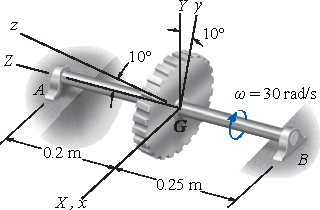
\includegraphics[width=\textwidth]{figures/hibb_21-4}
	\end{minipage}


	\item 
	\begin{minipage}[t][4.6cm]{0.55\textwidth}
		\textbf{Flywheel}
		The flywheel centered at \(G\) has a mass of \SI{10}{\kilo\gram} and is integral with the shaft of negligible mass that rotates at constant angular velocity \(\omega_s= \SI{6}{\per\second} \) (radians per second) supported by bearings \(A\) and \(B\).
		The first is a thrust bearing, so it provides reaction also in the longitudinal direction of the shaft, while the second only does so in the transverse directions.
		A transverse shaft to that of the flywheel supports the mount of bearing \(A\) and also rotates at constant angular velocity \(\omega_p\).
		\begin{tasks}
			\task Determine the reactions provided by the bearings.
		\end{tasks}
	\end{minipage}
	\begin{minipage}[c][0.5cm][t]{0.4\textwidth}
		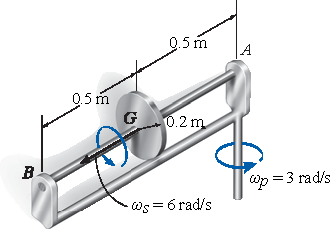
\includegraphics[width=\textwidth]{figures/hibb_21-6}
	\end{minipage}


	\item
	\begin{minipage}[t][3cm]{0.75\textwidth}
		\textbf{Off-axis Rotation}
		A homogeneous cylinder of mass \(m\), radius \(R\) and height \(H\) rotates at constant angular velocity \(\vec{\omega}\) around an axis that forms an angle of \ang{30;;} with the \(\hat{z}\) and passes through its center of mass.
		\begin{tasks}
			\task Calculate the torque that must be applied to the cylinder to maintain such motion.\\
			Result: \(
			\vec{\tau} = \left[\begin{matrix}\frac{\sqrt{3} m \omega^{2} \left(- H^{2} + 3 R^{2}\right)}{48}\\0\\0\end{matrix}\right]
			\) 
		\end{tasks}
	\end{minipage}
	\begin{minipage}[c][2cm][t]{0.2\textwidth}
		\includegraphics[width=\textwidth]{figures/Ex3_17}
	\end{minipage}



	\item 
	\begin{minipage}[t][4.5cm]{0.75\textwidth}
		\textbf{Rotating Rod}
		The thin rod AB has mass \(m\) and is connected to the support by means of a pin at A.
		The support is rigidly mounted on the shaft.
		Determine the required constant angular velocity \(\omega\) of the shaft so that the rod forms an angle \(\theta\) with the vertical.
	\end{minipage}
	\begin{minipage}[c][3cm][t]{0.2\textwidth}
		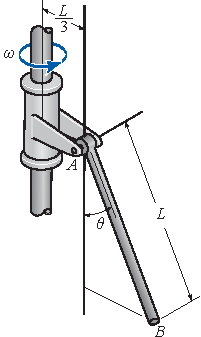
\includegraphics[width=\textwidth]{figures/hibb_21-45}
	\end{minipage}


	\item 
	\begin{minipage}[t][3.5cm]{0.6\textwidth}
	\textbf{Unbalanced Cylinder}
		A cylinder of height \(D\) and mass \(M\) rotates supported on two bearings \(P\) and \(Q\) with angular velocity \(\omega\).
		On an imaginary axis at an angle \(\varphi\) from the rotation axis, and at a distance \(a\) from its center, it has two weights of equal mass, \(m\), placed on it. 
		\begin{tasks} 
			\task Calculate the force applied by the bearings.\\
			Result: \(
				F = \frac{m a^2 \omega^2}{D} \sin(\varphi) \cos(\varphi)
			\).
		\end{tasks}
	\end{minipage}
	\begin{minipage}[c][0.5cm][t]{0.35\textwidth}
		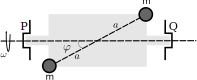
\includegraphics[width=\textwidth]{figures/cilindroDesbalanceado}
	\end{minipage}
		

	\item 
	\begin{minipage}[t][4.5cm]{0.55\textwidth}
		\textbf{Shaft on Bearings}
		The shaft was constructed with a rod whose mass per unit length is \SI{2}{\kilo\gram\per\metre}.
		Determine the \(x, y, z\) components of the reaction at bearings A and B if at the instant shown the shaft rotates freely at an angular velocity of \(\omega = \SI{30}{\per\second}\) (radians per second).
		What is the angular acceleration of the shaft at this instant?
		Bearing A is capable of supporting a force component in the y direction while bearing B is not.
	\end{minipage}
	\begin{minipage}[c][0cm][t]{0.4\textwidth}
		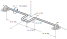
\includegraphics[width=\textwidth]{figures/hibb_21-48}
	\end{minipage}


	\item 
	\begin{minipage}[t][7cm]{0.65\textwidth}
		\textbf{Constant Angular Acceleration}
		The 15-pound cylinder rotates around axis AB with \(\vec{\omega} = -\SI{4}{\per\second} \hat{x}\) (radians per second).
		Bearing \(A\) does not support force in the \(x\) direction, which is handled by bearing \(B\).
		The shaft that extends from the support at point \(C\), starting from rest, is subjected to an acceleration \(\vec{\alpha}_C = \dot{\vec{\omega}} = \SI{12}{\per\second\squared} \hat{Z}\) (radians per second squared), where \(\hat{Z}\) includes \(\overline{AC}\) and is parallel to \(\hat{z}\).
		The coordinate system has its origin at \(G\), the center of mass of the cylinder.
		\begin{tasks}
			\task Convert the data in imperial units (feet, pounds) to International System units.
			\task Determine the reactions that the bearings must provide.\\
			Result: \(
			\left[\begin{matrix}A_{y}\\A_{z}\\B_{x}\\B_{y}\\B_{z}\end{matrix}\right] = \left[\begin{matrix}-5.79\\21.1 t + 33.4\\0\\5.79\\33.4 - 21.1 t\end{matrix}\right]
			\)
		\end{tasks}
	\end{minipage}
	\begin{minipage}[c][2cm][t]{0.3\textwidth}
		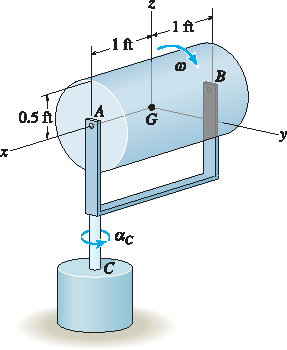
\includegraphics[width=\textwidth]{figures/hibbEng_21-58}
	\end{minipage}


	\item 
	\begin{minipage}[t][3.5cm]{0.65\textwidth}
		\textbf{Rock Crusher}
		A rock crusher consists of a large thin disk which is connected by means of a pin to a horizontal shaft.
		If it rotates at a constant speed of \SI{8}{\per\second} (radians per second), determine the normal force that the disk exerts on the stones.
		Assume that the disk rolls without slipping and that its mass is \SI{25}{\kilo\gram}.
		Ignore the mass of the shaft.
	\end{minipage}
	\begin{minipage}[c][2cm][t]{0.3\textwidth}
		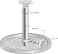
\includegraphics[width=\textwidth]{figures/hibb_21-56}
	\end{minipage}


\end{enumerate}

\end{document}